\documentclass[10pt, aspectratio=169]{beamer}
\usepackage[T1]{fontenc}
\usepackage{helvet}
\renewcommand{\familydefault}{\sfdefault}
\usepackage{booktabs}
\usepackage{graphicx}

% ----------------------------------------------------
% CUSTOM GSAPP MINIMAL TIER
% ----------------------------------------------------
\setbeamertemplate{navigation symbols}{}
\setbeamercolor{background canvas}{bg=white}
\setbeamercolor{normal text}{fg=black}
\setbeamercolor{frametitle}{fg=black, bg=white}
\setbeamercolor{title}{fg=black}
\setbeamercolor{subtitle}{fg=black!70}
\setbeamercolor{author}{fg=black!60}
\setbeamercolor{itemize item}{fg=black}
\setbeamertemplate{itemize item}{\rule[0.3ex]{0.8ex}{0.8ex}}

% Clean, massive frame titles with heavy bottom padding
\setbeamertemplate{frametitle}{
    \vspace{1.2em}
    \usebeamerfont{frametitle}\huge\textbf{\insertframetitle}
    \vspace{0.4em}
}

% Bespoke GSAPP Title Page resolving the parenthetical bug.
\setbeamertemplate{title page}{
    \vspace{4.5em}
    {\huge\textbf{\inserttitle}\par}
    \vspace{1em}
    {\Large\textcolor{black!70}{\insertsubtitle}\par}
    \vspace{3.5em}
    {\large\insertauthor\par}
    {\normalsize\textcolor{black!60}{Graduate School of Architecture, Planning and Preservation\\Columbia University}\par}
    \vspace{1.5em}
    {\normalsize\textcolor{black!60}{\insertdate}\par}
}
% ----------------------------------------------------

\title{Predicting Formal Protest Petitions Against Housing Development}
\subtitle{Evidence from Austin, Texas}
\author{Daniel Hardesty Lewis \\ M.S. Candidate, Urban Planning}
\date{April 16, 2026}

% Graphic paths matching the main document
\graphicspath{{Figures/}{../../Analysis/Output/}}

\begin{document}

\begin{frame}[plain]
    \titlepage
\end{frame}

\begin{frame}{Institutionalized NIMBYism}
    \begin{columns}
        \column{0.5\textwidth}
        \textbf{The 20\% Threshold}
        \vspace{1em}
        
        If owners of 20\% of the land within 200 feet of a proposed rezoning file written opposition, City Council requires a \textbf{supermajority (3/4)} vote to approve it.
        \vspace{1em}
        
        \textit{This effectively gives small groups of nearby owners veto power over citywide housing decisions.}
        
        \column{0.5\textwidth}
        \centering
        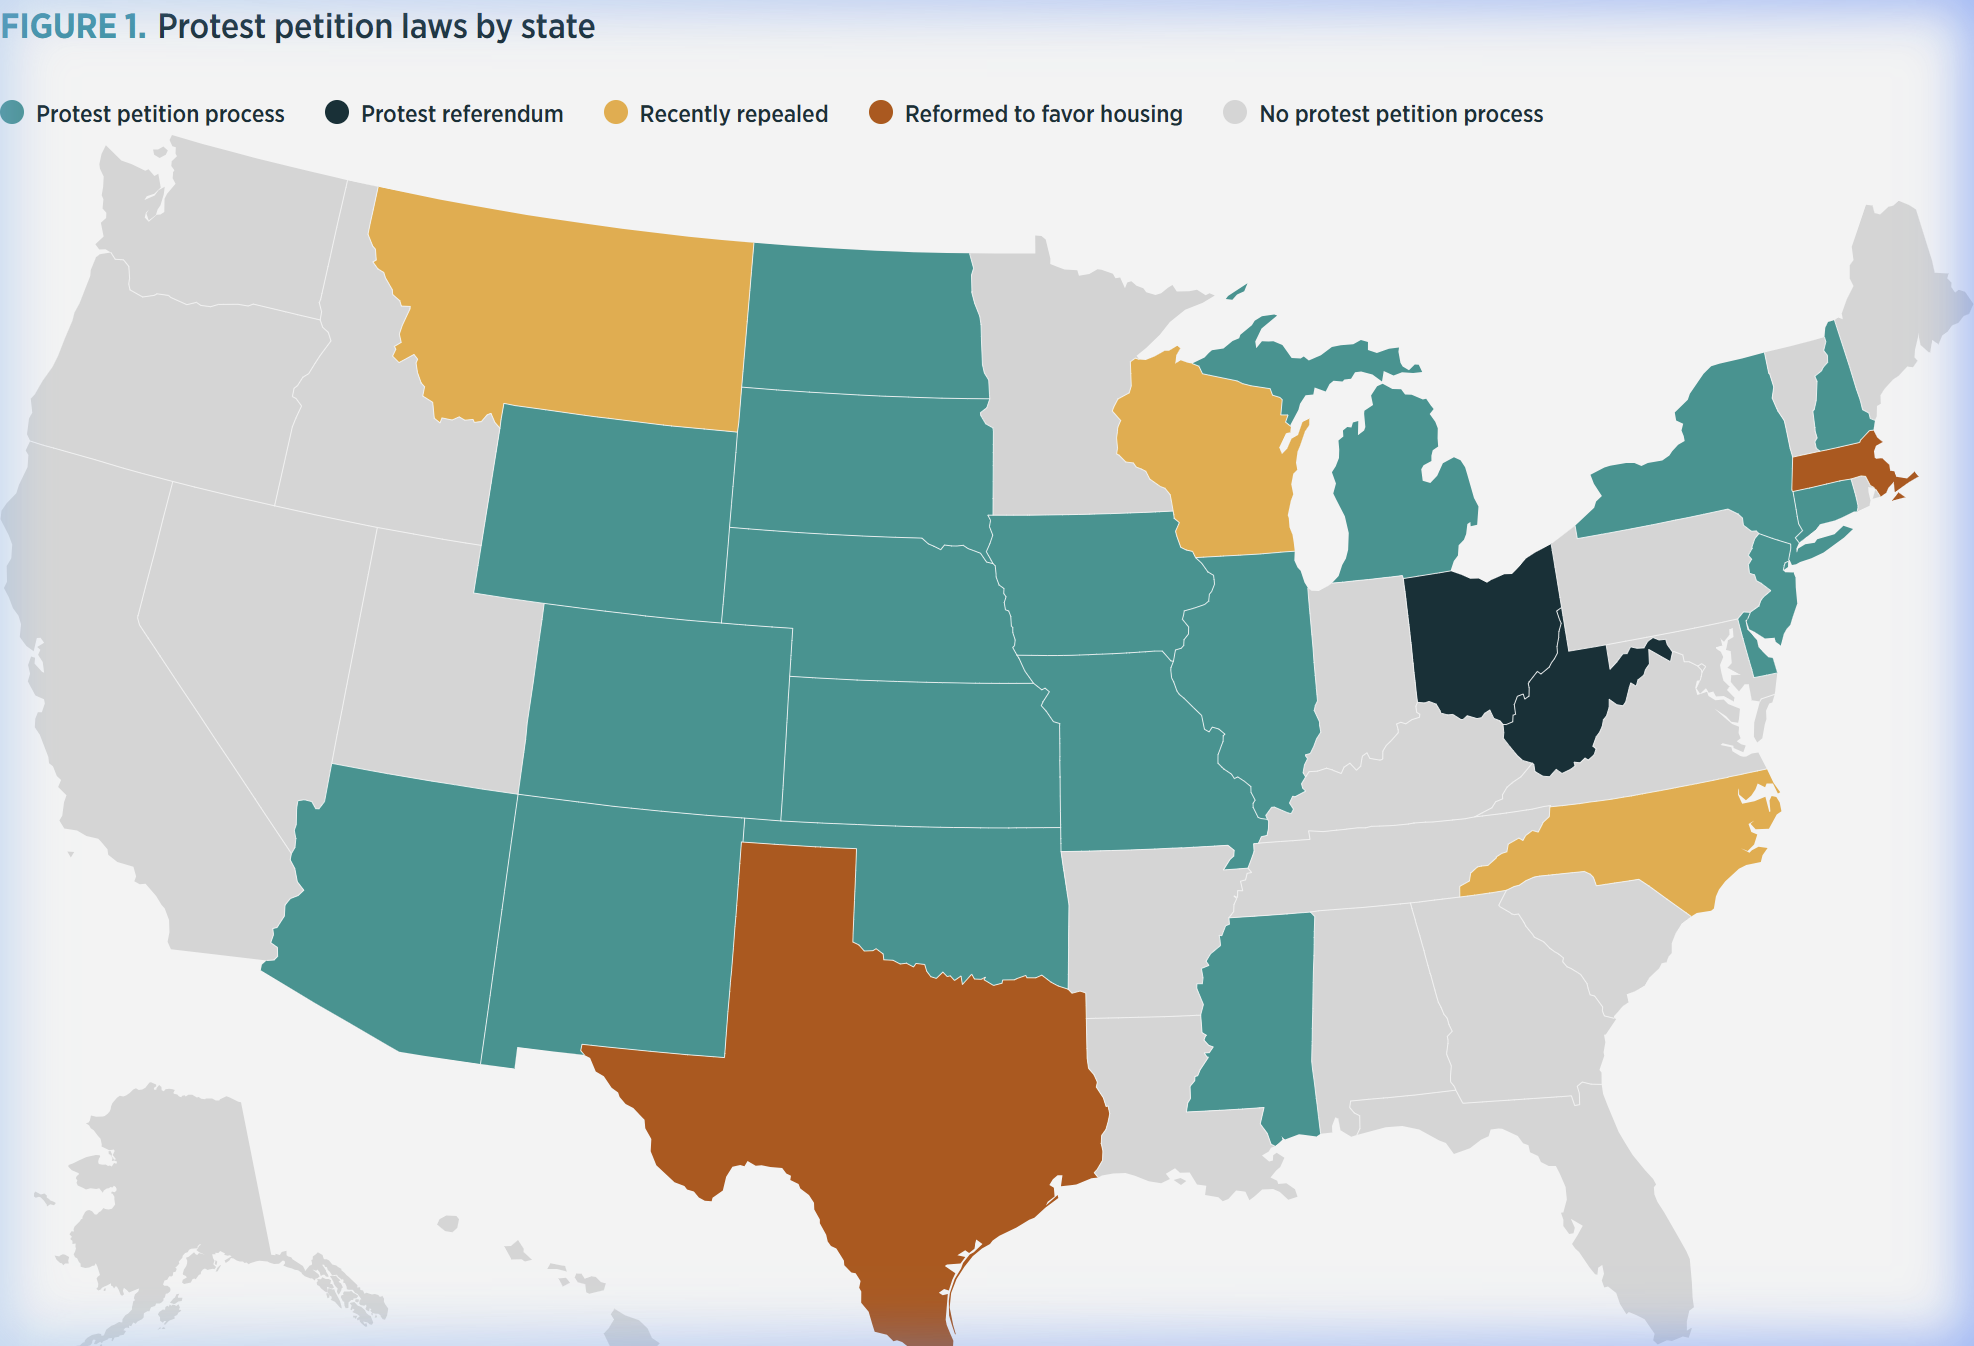
\includegraphics[width=\linewidth, height=0.75\textheight, keepaspectratio]{exhibits/mercatus_map.png}
    \end{columns}
\end{frame}

\begin{frame}{Statutory Context: The Institutional Veto}
    \begin{columns}
        \column{0.5\textwidth}
        \textbf{Texas LGC Chapter 211}
        \begin{itemize}
            \item \textbf{The 20\% Rule}: If owners of 20\% of the land within 200ft sign a valid protest, a \textit{supermajority} vote is required.
            \item \textbf{High-Stakes Voting}: In a 7-member council, this moves from 4 votes to 6.
            \item \textbf{Asymmetric Veto}: A localized minority can block citywide housing policy through formal administrative friction.
        \end{itemize}
        
        \column{0.5\textwidth}
        \centering
        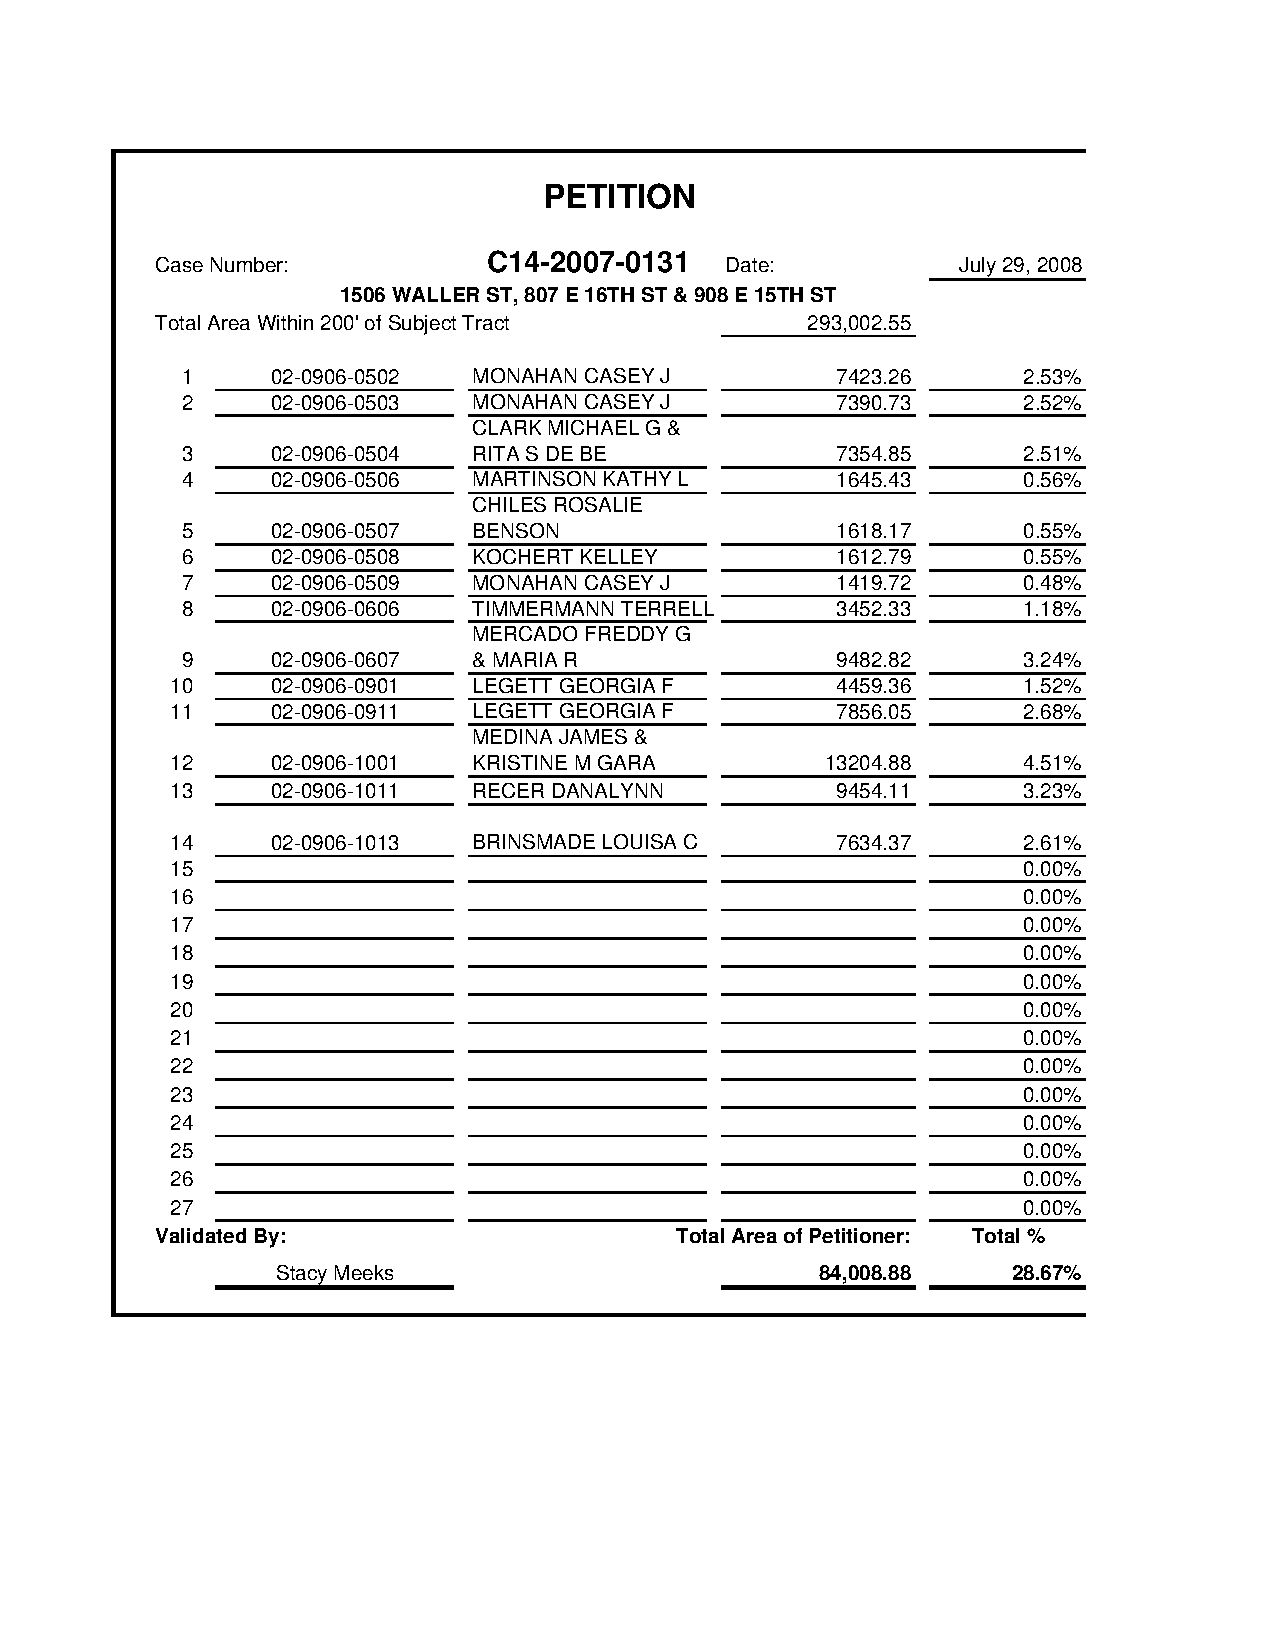
\includegraphics[width=0.9\textwidth]{appendix/fig_app_04_sample_protest_petition_v15.pdf} \\
        \footnotesize \textit{Sample Formal Protest Petition Record}
    \end{columns}
\end{frame}

\begin{frame}{The Goal and The Data}
    \begin{columns}
        \column{0.5\textwidth}
        \textbf{The Research Question}
        \vspace{0.5em}
        {\large Can we anticipate formal protest petitions \textit{before} public hearings?}
        
        \vspace{1.5em}
        \textbf{Filing-Date Records}
        \begin{itemize}
            \item Site area, height/FAR deltas.
            \item Current vs requested zoning.
            \item Neighborhood spatial context.
        \end{itemize}
        
        \column{0.5\textwidth}
        \textbf{A Sample Case}
        \vspace{1em}
        {\footnotesize
        \begin{tabular}{ll}
            \toprule
            Feature & Case C14-2018-0156 \\
            \midrule
            Gross Site Area & 4.92 Acres \\
            Height Request & +15.5 ft \\
            FAR Request & +0.43 \\
            Neighborhood & Riverside \\
            \textbf{Result} & \textbf{Valid Petition} \\
            \bottomrule
        \end{tabular}
        }
    \end{columns}
\end{frame}

\begin{frame}{Technical Pipeline: Data Generation}
    \begin{columns}
        \column{0.5\textwidth}
        \textbf{As-Of Context Reconstruction}
        \begin{itemize}
            \item \textbf{Data Recovery}: Reconstructing 15+ years of zoning agendas.
            \item \textbf{Parsing Pipelines}: PDF scraping of Clerk records.
            \item \textbf{Timeline Integrity}: Ensuring no ``future leakage'' (predicting only with data available at filing).
            \item \textbf{Expert Grounding}: Semi-structured interviews ($N=8$) with planners and advocates to calibrate model interpretations.
        \end{itemize}
        
        \column{0.5\textwidth}
        \centering
        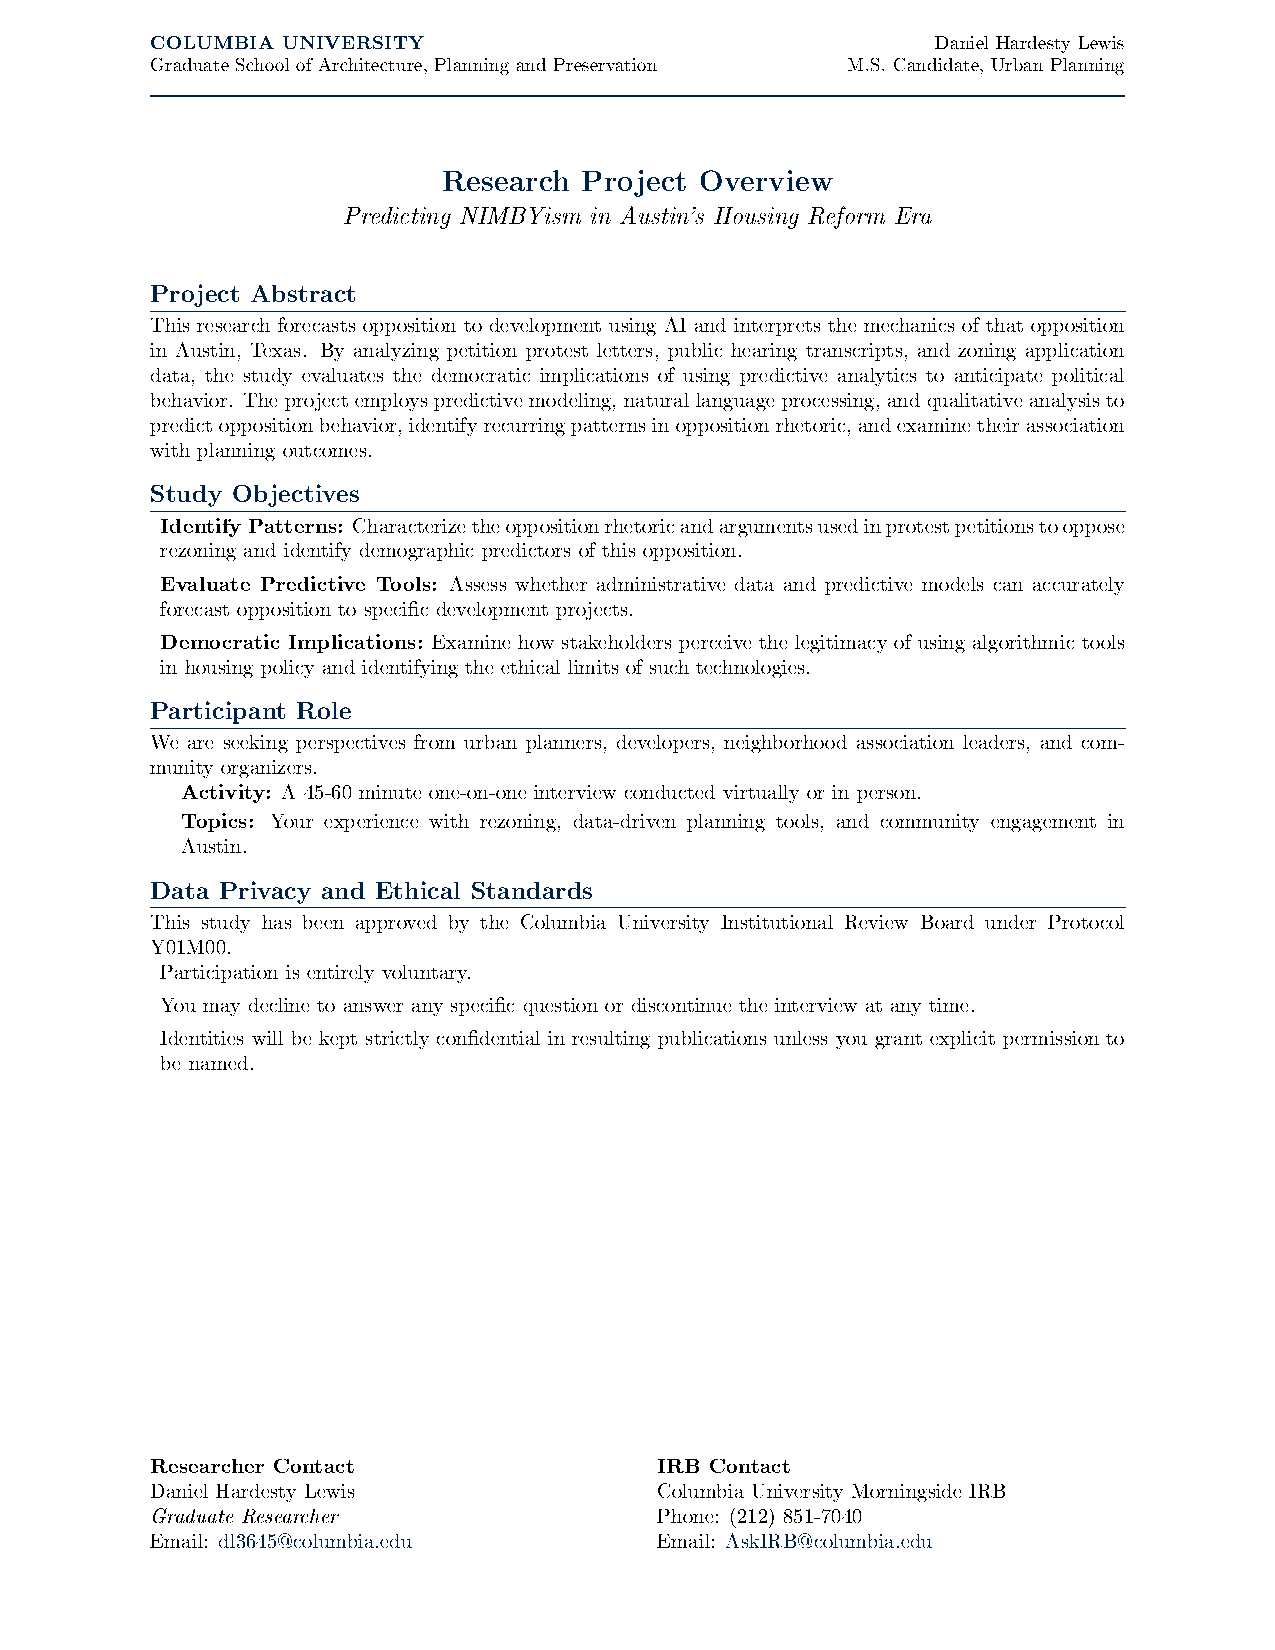
\includegraphics[width=0.9\textwidth]{appendix/fig_app_02_project_overview.pdf}
    \end{columns}
\end{frame}

\begin{frame}{The Rarity Problem}
    \begin{columns}
        \column{0.4\textwidth}
        \textbf{Sample Constraints}
        \begin{itemize}
            \item \textbf{Universe}: 2007--2024 Austin rezonings.
            \item \textbf{Distribution}: $\approx 2.6\%$ baseline petition rate.
            \item \textbf{Evaluation}: Strictly temporal (forward-looking) holdouts.
        \end{itemize}
        
        \column{0.6\textwidth}
        \centering
        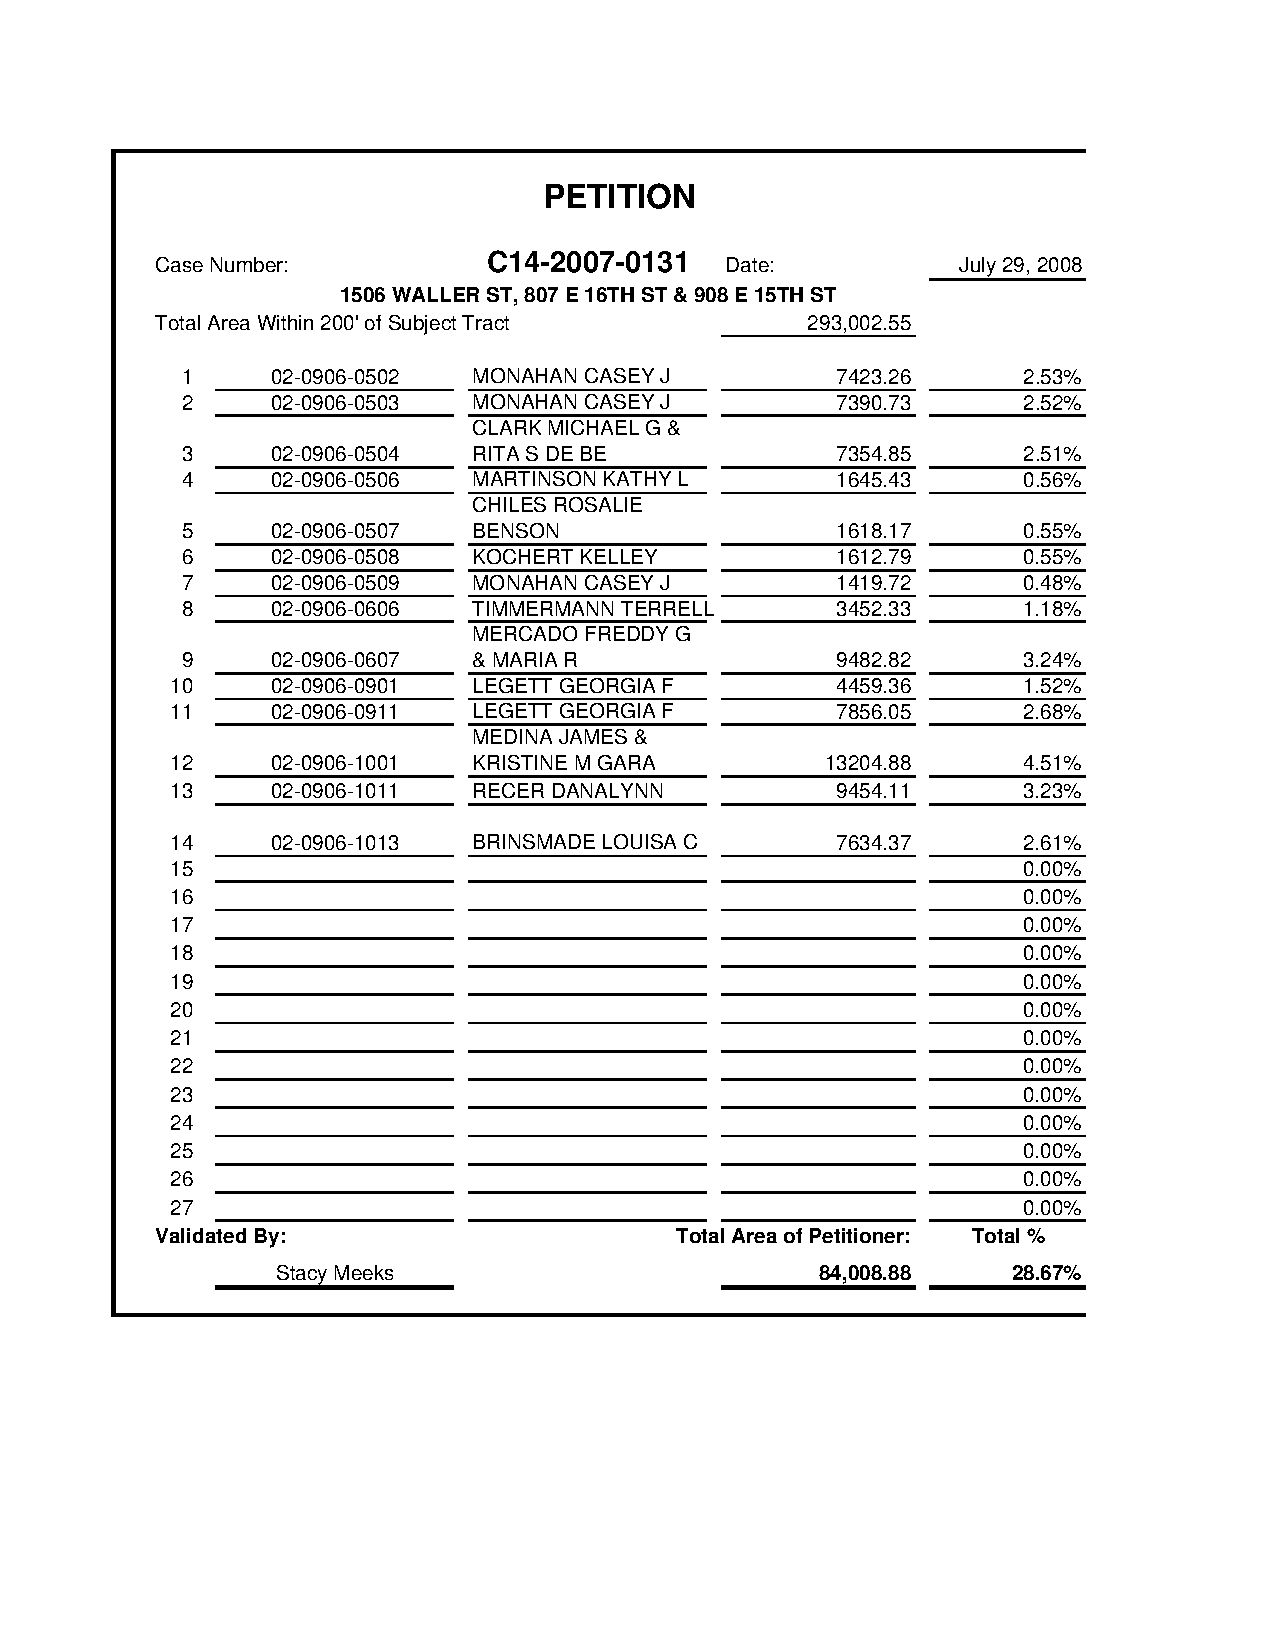
\includegraphics[height=0.75\textheight, width=\linewidth, keepaspectratio]{appendix/fig_app_04_sample_protest_petition_v15.pdf}
    \end{columns}
\end{frame}

\begin{frame}{Predicting Resistance}
    \centering
    \textbf{Trees Dominate at the Top of the Ranking}
    \vspace{1em}
    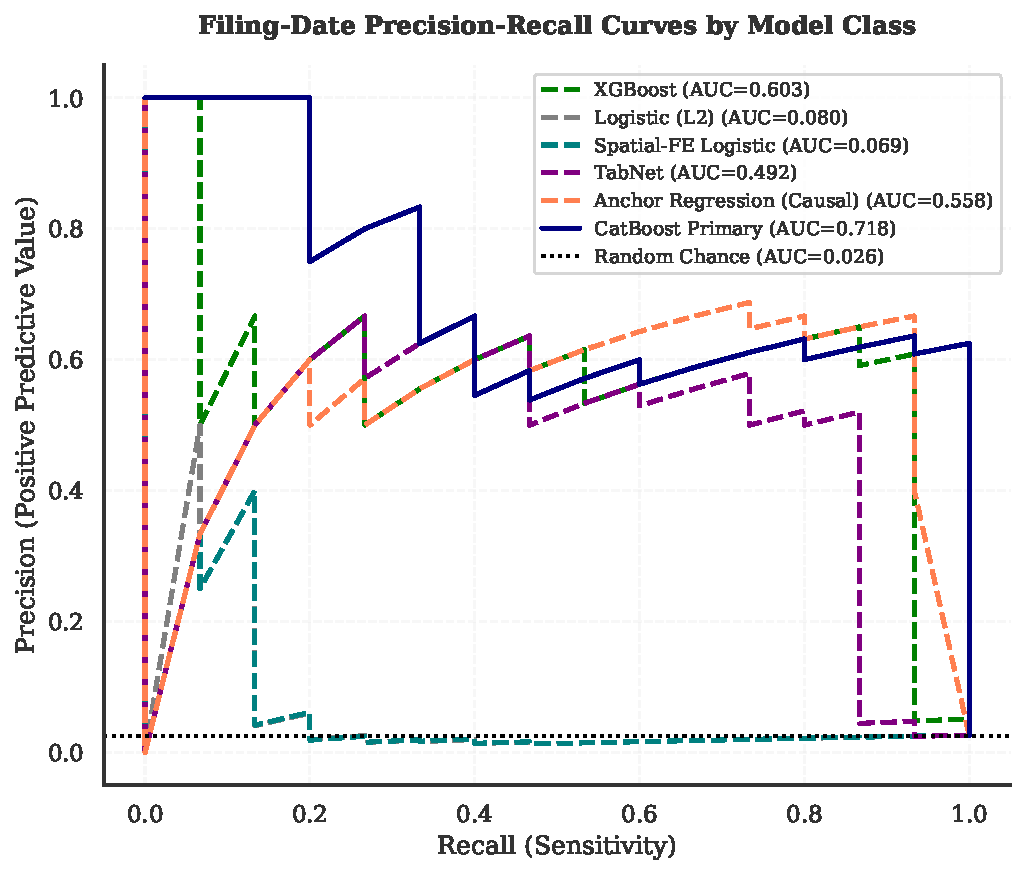
\includegraphics[height=0.70\textheight, width=\textwidth, keepaspectratio]{exhibits/fig_pr_curves_updated.pdf}
\end{frame}

\begin{frame}{Modeling Architectures: Benchmarking}
    \begin{columns}
        \column{0.5\textwidth}
        \textbf{CatBoost vs. TabNet}
        \begin{itemize}
            \item \textbf{Tree Ensembles}: Robust to diverse feature scales; dominant in tabular planning data.
            \item \textbf{Deep Architectures}: High sensitivity to parameter tuning; struggle with discrete spatial boundaries.
            \item \textbf{The Winner}: Tree-based models achieve 2X the precision in high-triage tiers.
        \end{itemize}
        
        \column{0.5\textwidth}
        \centering
        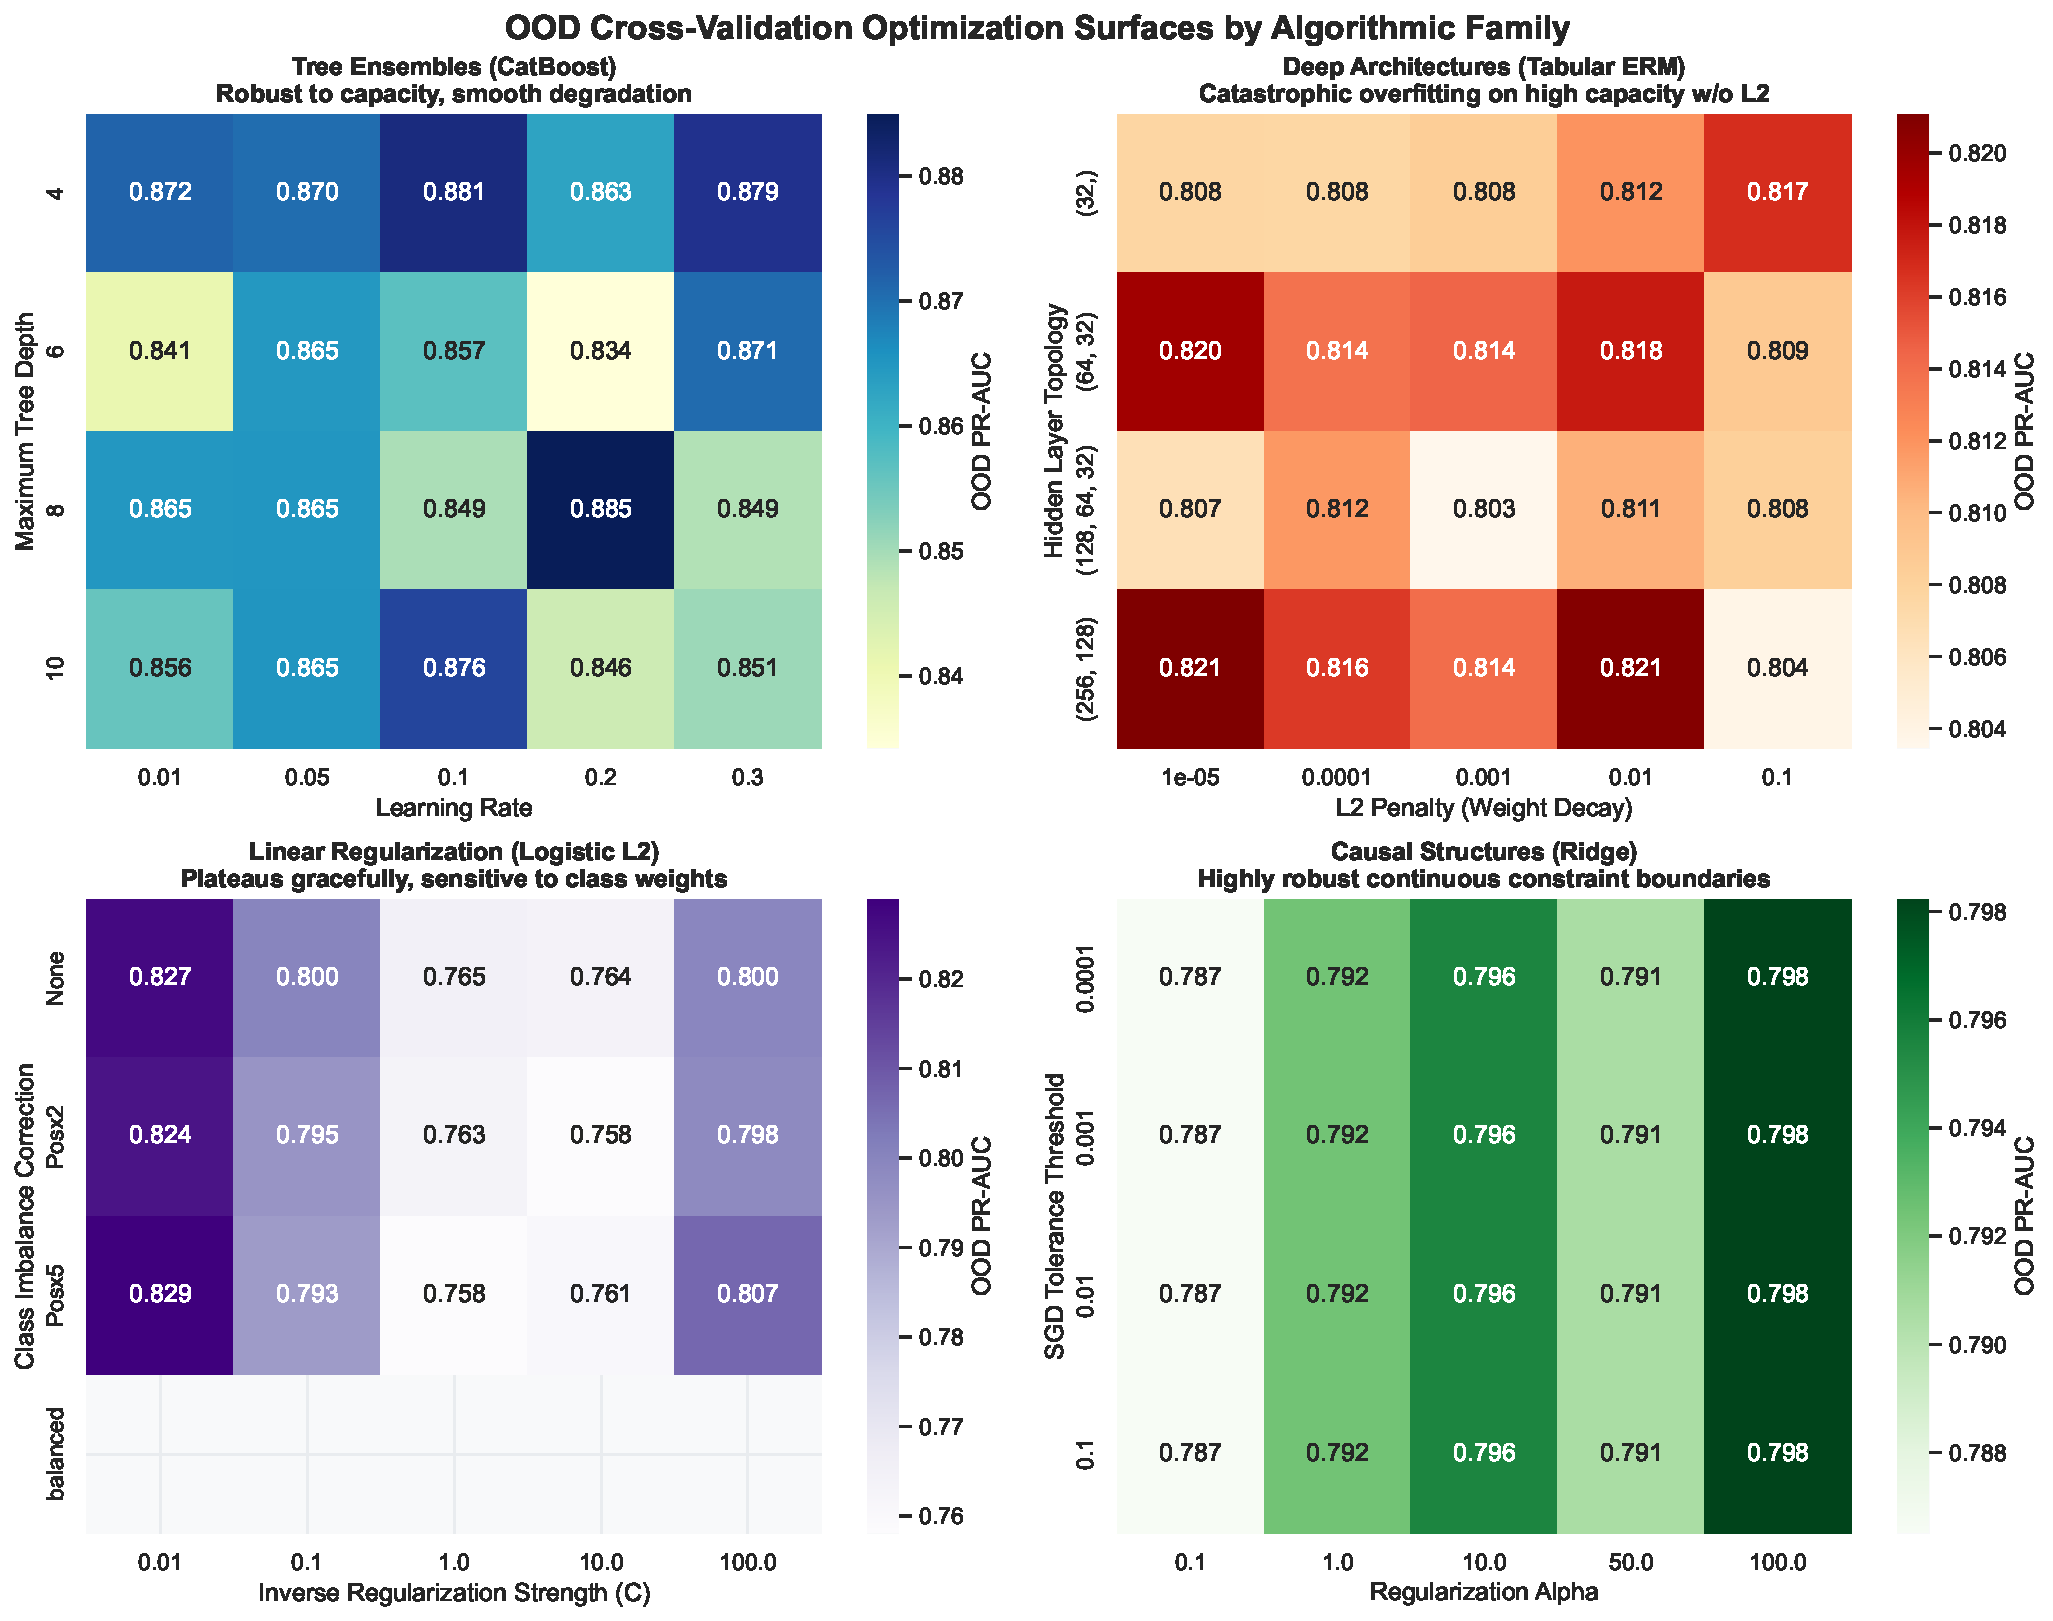
\includegraphics[width=0.9\textwidth]{exhibits/fig_hyperparameter_sweeps_benchmark.pdf}
    \end{columns}
\end{frame}

\begin{frame}{Dealing with Collinearity}
    \begin{columns}
        \column{0.4\textwidth}
        \textbf{Semantic Clustering}
        \vspace{1em}
        
        Standard feature attribution fragments importance across collinear features because isolated real estate variables proxy identical physical concepts (e.g., site area, deed acreage).
        \vspace{1em}
        
        We sum absolute TreeSHAP values within semantic clusters of correlated features.
        
        \column{0.6\textwidth}
        \centering
        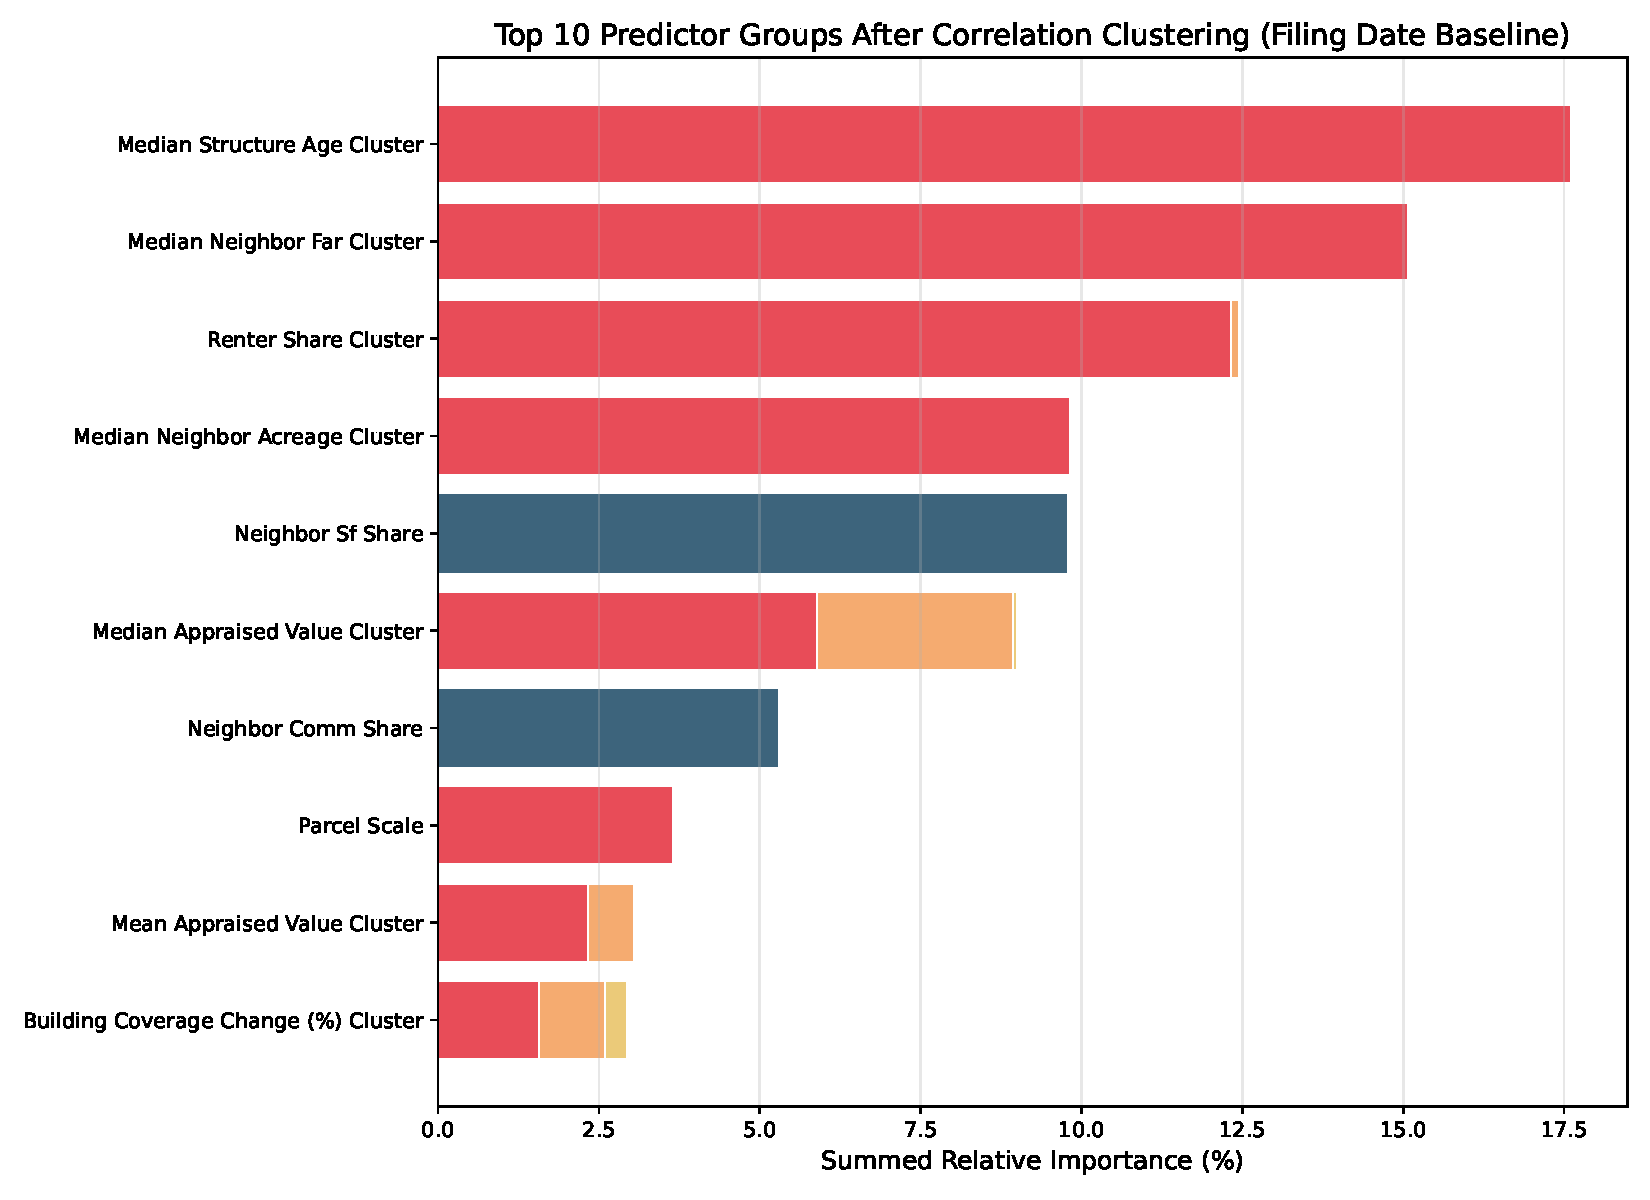
\includegraphics[height=0.75\textheight, width=\linewidth, keepaspectratio]{exhibits/fig_feature_importance_clustered_H0_Full.pdf}
    \end{columns}
\end{frame}

\begin{frame}[plain]
    \centering
    \textbf{Architectural Separation of Feature Reliance}\\
    \vspace{0.5em}
    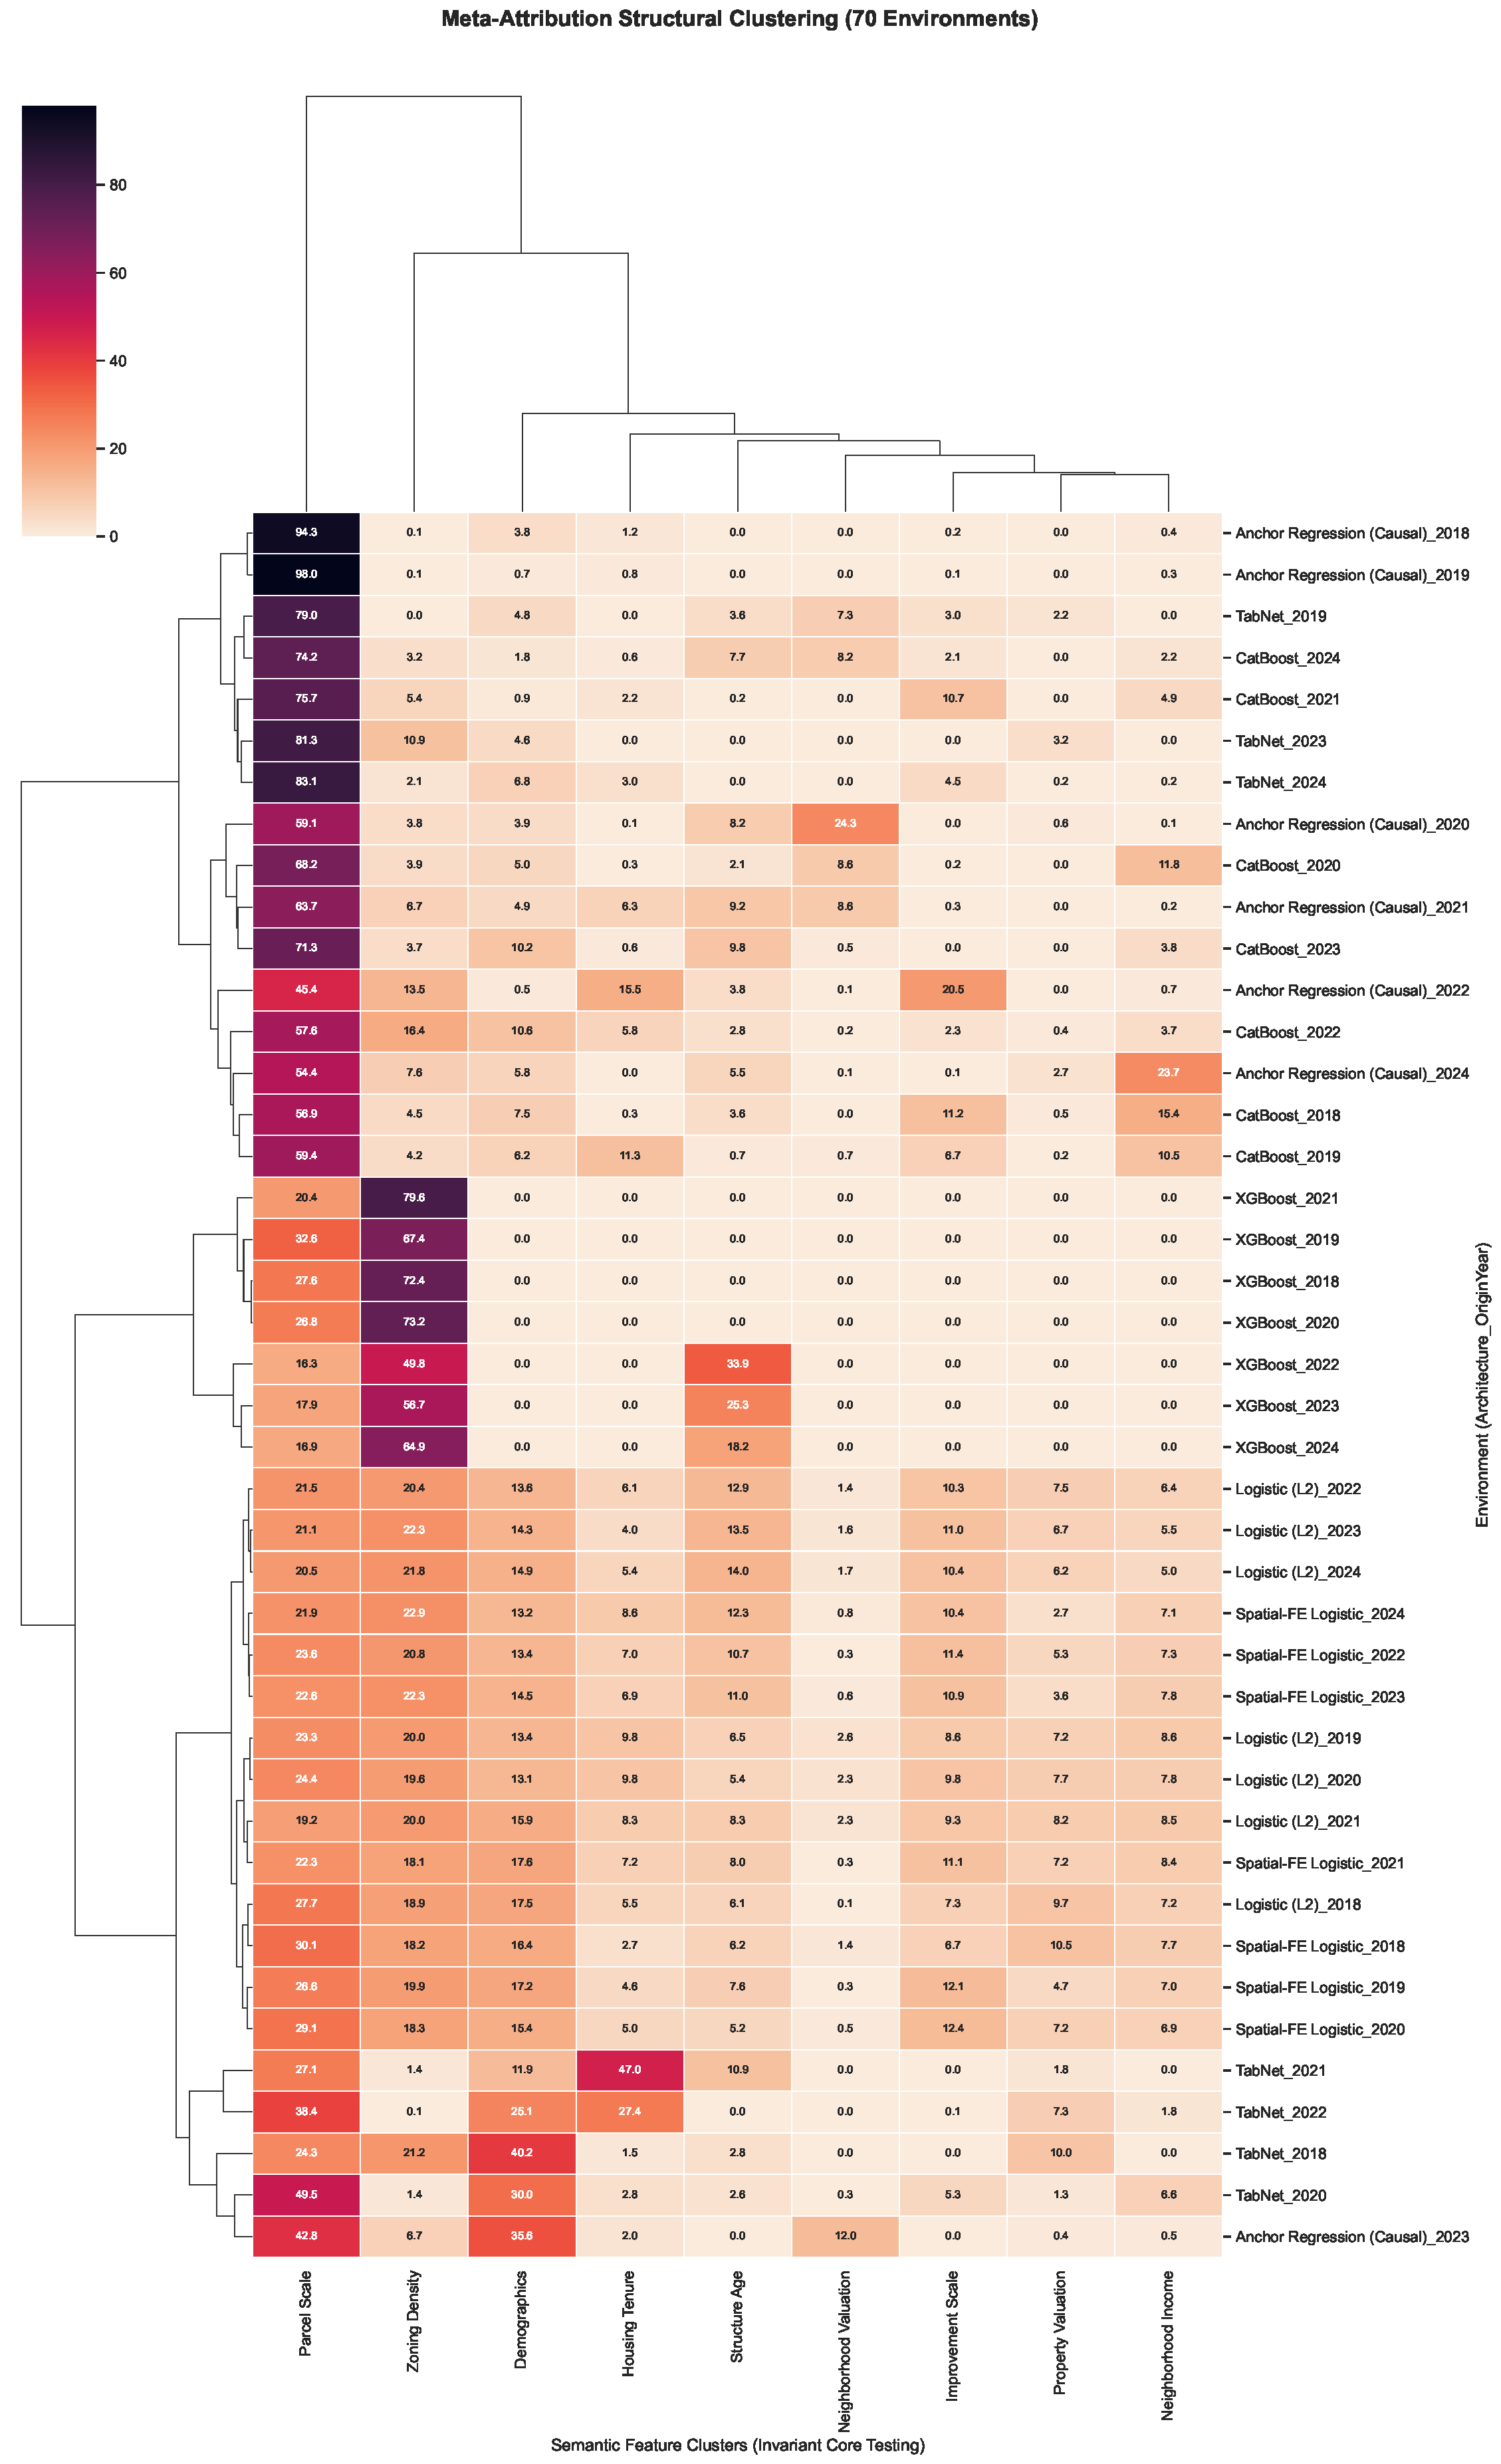
\includegraphics[height=0.8\textheight, width=\textwidth, keepaspectratio]{ch5/fig_ch5_35_meta_attribution_clustermap.pdf}
\end{frame}

\begin{frame}{Temporal Drift}
    \begin{columns}
        \column{0.5\textwidth}
        \textbf{When does the model break?}
        \vspace{1em}
        
        Historical models suffer from \textit{concept drift} when encountering modern low-conflict environments. 
        \vspace{1em}
        
        Linear models collapse entirely as the gap between training and test years widens, while Tree Ensembles degrade more gracefully.
        
        \column{0.5\textwidth}
        \centering
        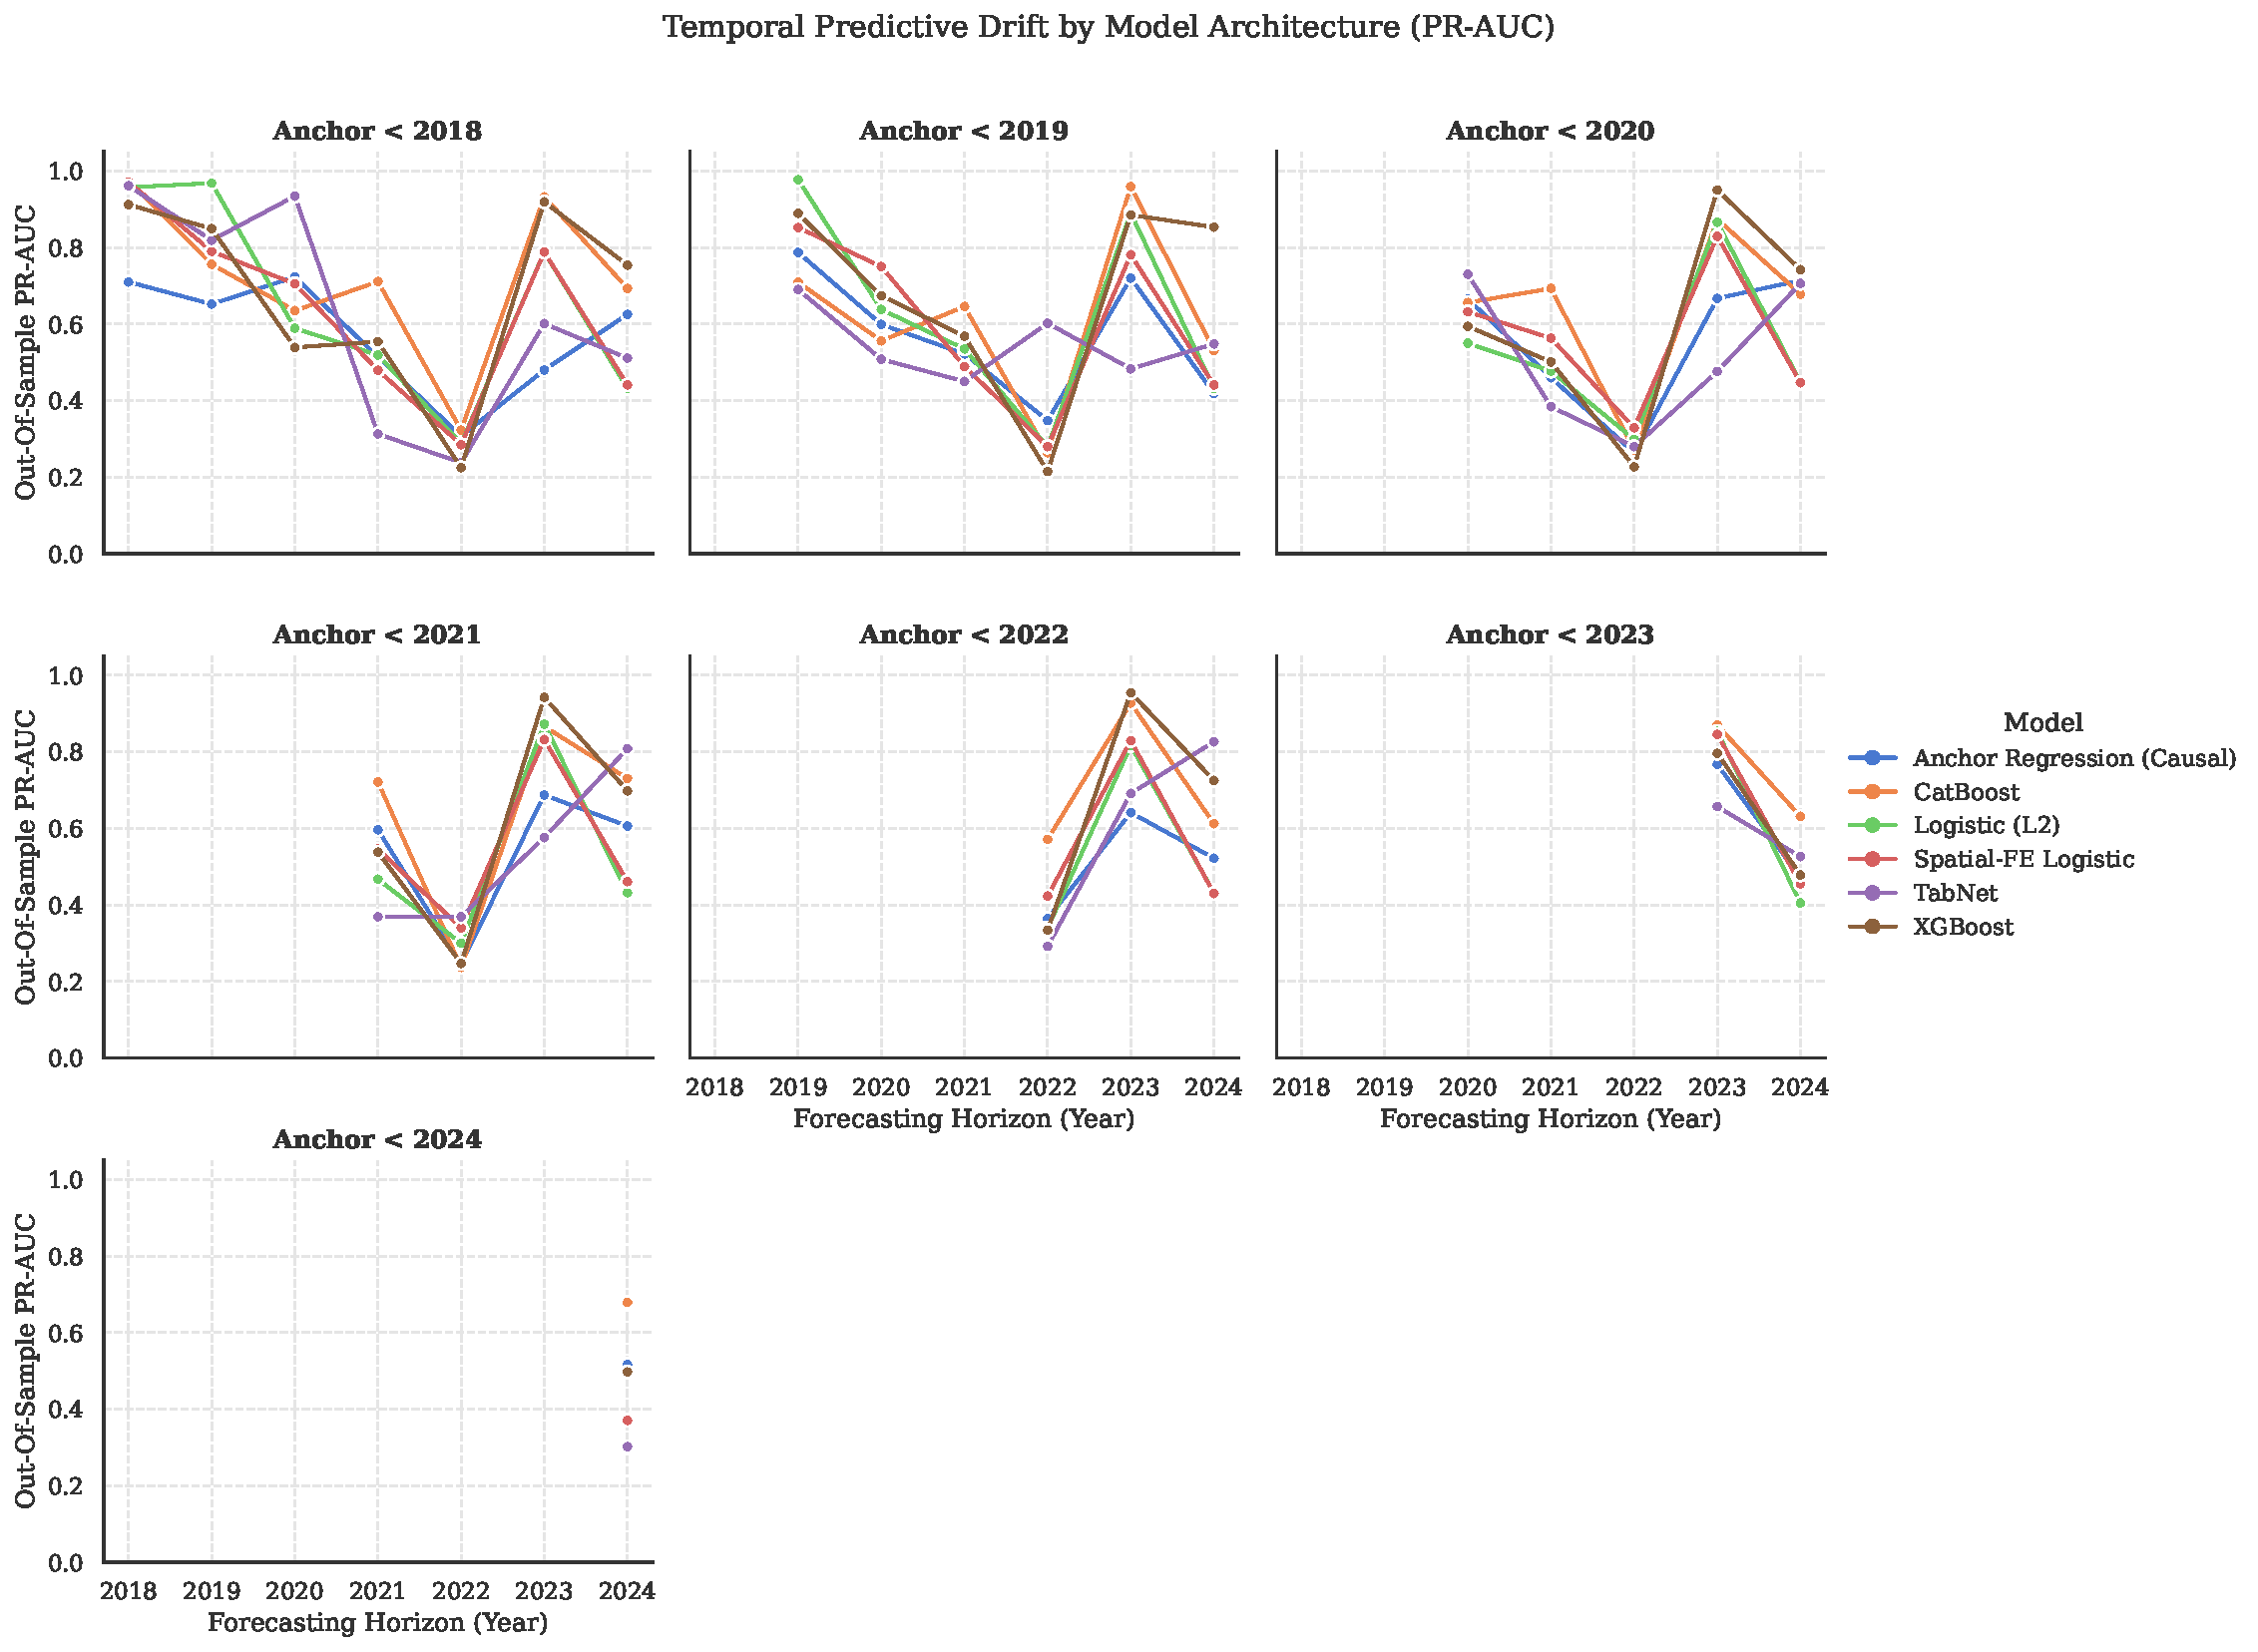
\includegraphics[width=\linewidth]{exhibits/fig_temporal_drift_prauc_testyear.pdf}
    \end{columns}
\end{frame}

\begin{frame}{Agency in Temporal Shifts}
    \begin{columns}
        \column{0.5\textwidth}
        \textbf{The 2022 Performance Dip}
        \begin{itemize}
            \item \textbf{The Finding}: Model performance plummeted in 2022 across all architectures.
            \item \textbf{Hypothesis}: Consistently low performance in 2022 align with pandemic-era filing shifts and administrative uncertainty.
            \item \textbf{Agency Proof}: Proves that predictability is not static, but contingent on social/political intelligence.
        \end{itemize}
        
        \column{0.5\textwidth}
        \centering
        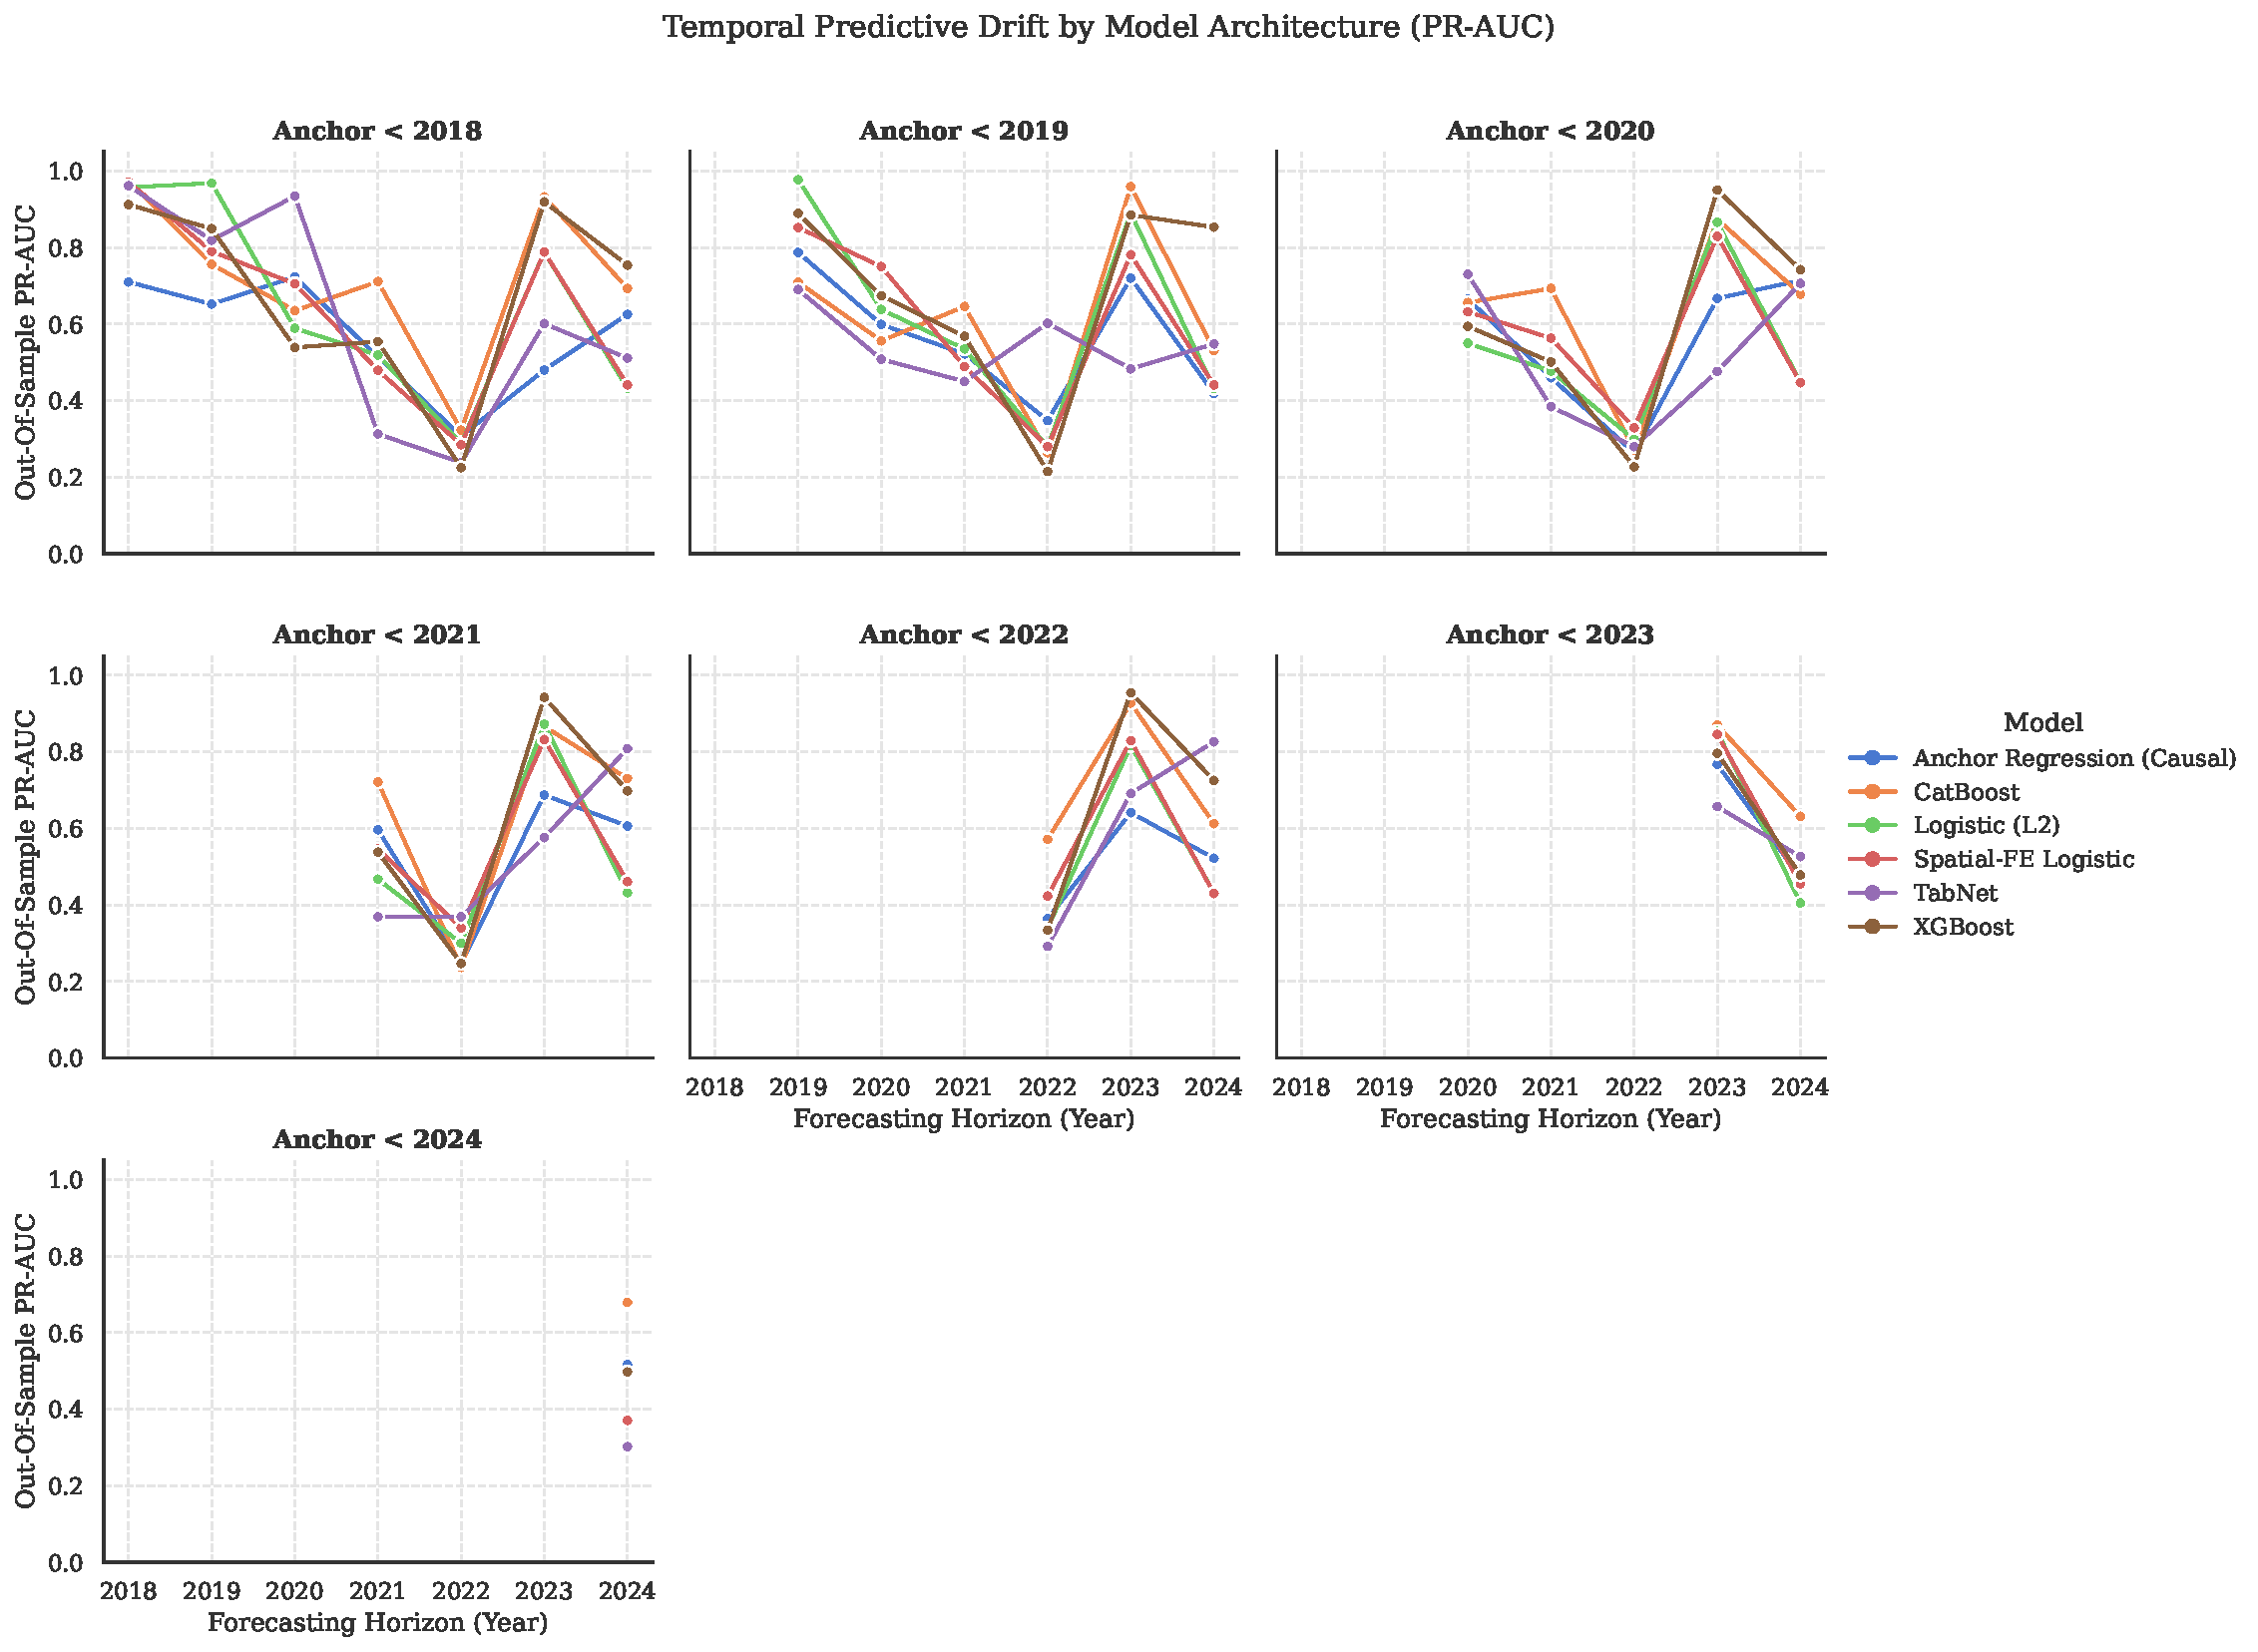
\includegraphics[width=\linewidth]{exhibits/fig_temporal_drift_prauc_testyear.pdf}
    \end{columns}
\end{frame}

\begin{frame}{Qualitative Context: Stakeholder Insights}
    \begin{columns}
        \column{0.6\textwidth}
        \textbf{The ``Motive Blindness'' Discovery}
        \begin{itemize}
            \item The algorithm cannot distinguish between \textbf{exclusionary NIMBYism} and \textbf{anti-displacement resistance}.
            \item Quantitative risk weights are independent of neighborhood intent or social equity goals.
        \end{itemize}
        
        \textbf{Expert Perspectives}
        \begin{itemize}
            \item \textit{``Haters are overrepresented and silent supporters are underrepresented''} (Beaudet).
            \item Algorithm fails \textit{``to identify where people that are in actual need actually are''} (Torrado).
            \item Professionals view rigid probability cutoffs as ``ethically hazardous.''
        \end{itemize}

        \column{0.4\textwidth}
        \centering
        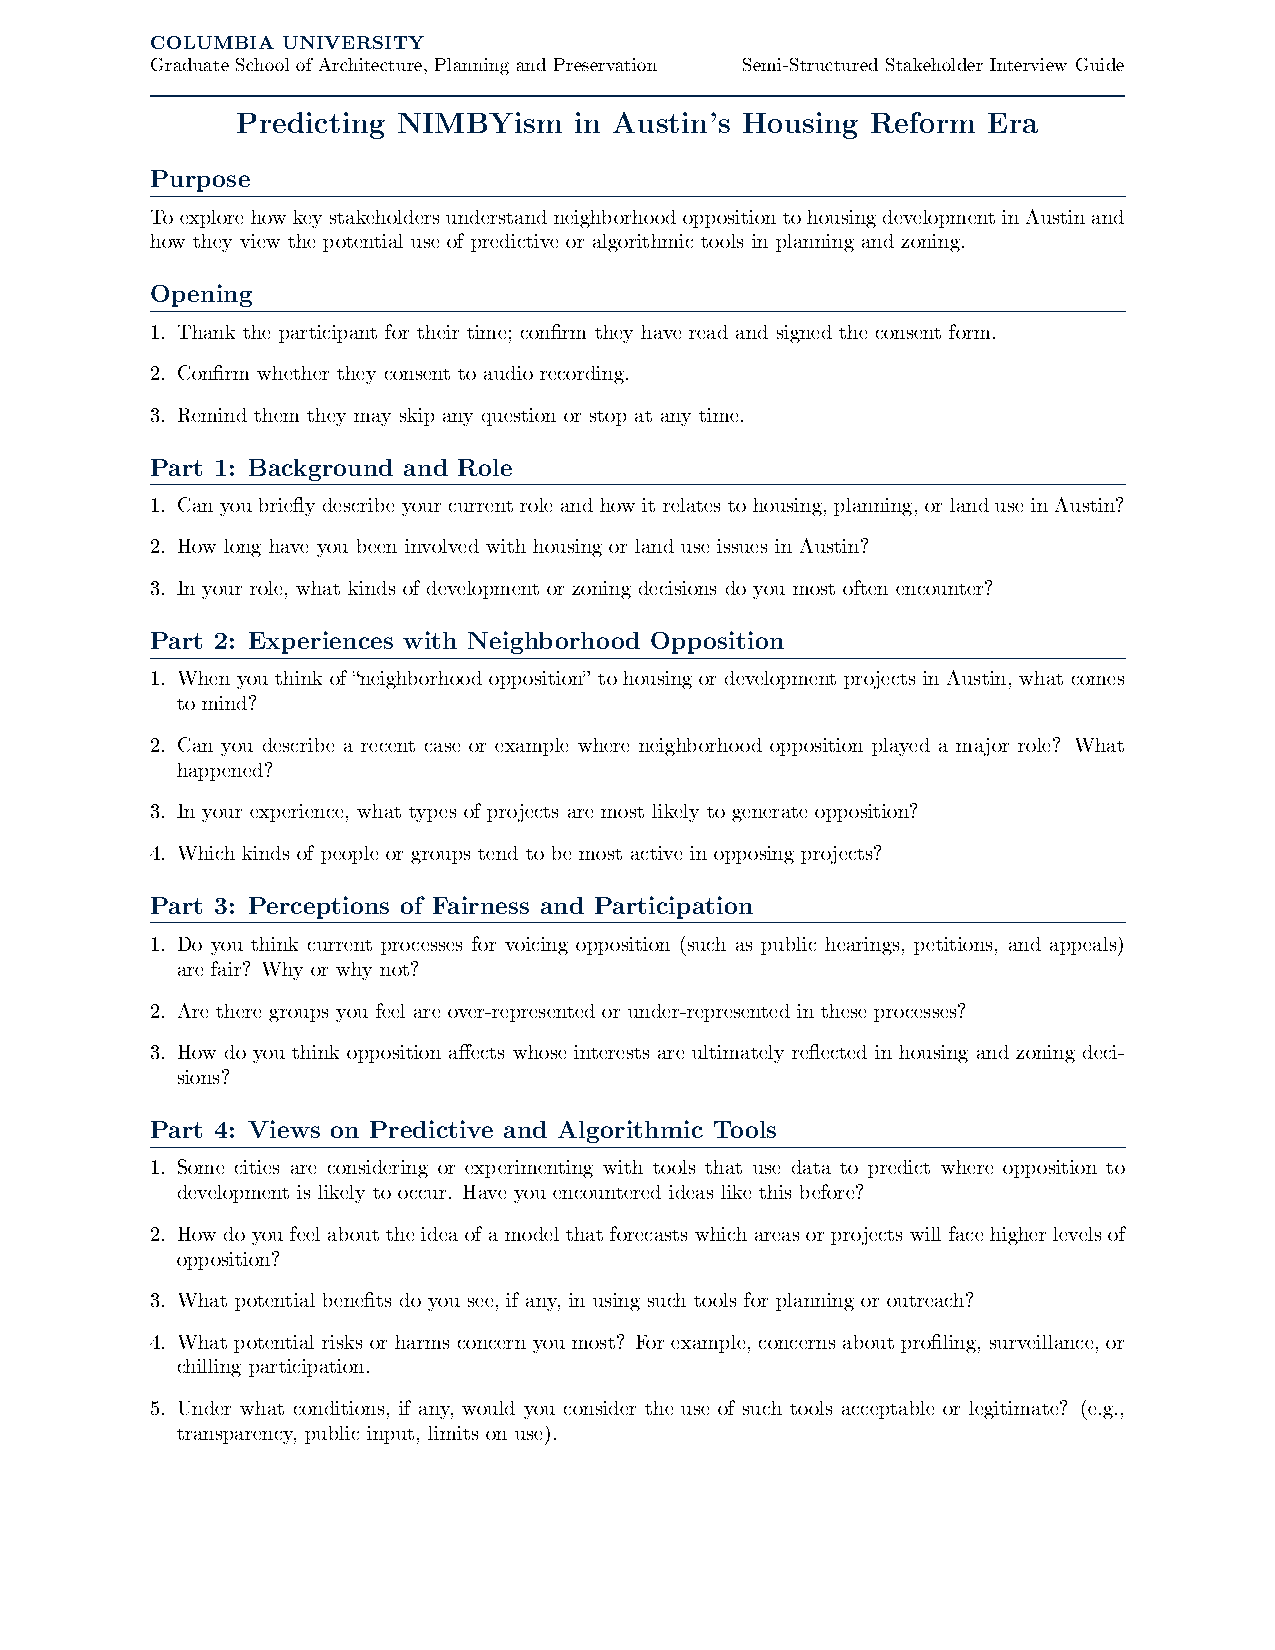
\includegraphics[width=\linewidth]{appendix/fig_app_01_interview_guide.pdf} \\
        \footnotesize \textit{Sample Interview Protocol}
    \end{columns}
\end{frame}

\begin{frame}{Conclusion}
    \small
    \textbf{What we showed}
    \begin{itemize}
        \item \textbf{Predictive Utility}: Filing-date administrative data carries real predictive signal (PR-AUC 0.724), \textbf{qualitatively validated by practitioners}.
        \item \textbf{Tree Dominance}: Ensemble methods consistently lead at the top of the risk ranking tier.
    \end{itemize}
    
    \textbf{What surprised us}
    \begin{itemize}
        \item \textbf{Observed Ceilings}: Model reliability is bounded by something other than longitudinal feature richness.
        \item \textbf{Defensible Agency}: Performance floors are consistent with mobilization being a \textbf{strategic choice} rather than a mechanical response to parcel spatiality.
    \end{itemize}

    \textbf{What it implies}
    \begin{itemize}
        \item \textbf{Decision Policy}: Algorithm selection is a non-technical choice about which urban feature clusters are prioritized.
    \end{itemize}
    
    \vspace{2em}
    \centering
    \rule{0.5\textwidth}{0.4pt} \\
    \footnotesize \textit{Ethics Warning: This model ranks risk; it should not be used to pre-screen sites for developers seeking the path of least resistance.}
\end{frame}

\begin{frame}{Implications: A Now-Closed Policy Window}
    \textbf{The HB 24 Shift (2025)}
    \begin{itemize}
        \item \textbf{Institutional Reform}: Texas HB 24 gutted the petition mechanism for residential upzonings.
        \item \textbf{Context Bound}: This thesis maps a specific, historical era of minority veto power.
        \item \textbf{Method Portability}: The methodology travels; the parameters remain Austin-specific.
    \end{itemize}
    
    \vspace{2em}
    \textit{This model identifies risk in a historical architecture; current policy has moved toward broad administrative deregulation.}
\end{frame}

\begin{frame}[plain]
    \centering
    \Huge \textbf{Discussion / Q\&A}
    \vspace{2em}
    
    \small \textit{Thank you to the committee for your time and feedback.}
\end{frame}

\begin{frame}[plain]
    \centering
    \vspace{2em}
    {\Huge\textbf{Thank You}}
    \vspace{1.5em}
    
    {\small To all who advised, read, and commented on my thesis}
    \vspace{2em}
    
    Dory Kornfeld \\
    \vspace{0.5em}
    Weiping Wu \\
    \vspace{0.5em}
    James Piacentini \\
    \vspace{0.5em}
    Stijn Van Nieuwerburgh \\
    \vspace{0.5em}
    Matthew Bauer \\
    \vspace{0.5em}
    Adam Vosburgh \\
    \vspace{0.5em}
    Josh Begley
\end{frame}

\end{document}
